\section{Zhodnotenie výsledkov}\label{sec:experiments}
S popísanými algoritmami boli vykonávané experimenty pre overenie správnosti navrhnutých štruktúr a nájdenie možných
vzorcov vo výsledkoch.
Kľúčovou informáciou je počet výhier hráča \textbf{X} (resp. podiel výhier vzhľadom na počet hier) v prípade
umelých neurónových sietí; čas a výhra v prípade algoritmu MinMax.

\subsection{Experimenty s rôznymi plochami}\label{subsec:experiments-board}

Experimenty boli vykonávané v 2 variantoch:
\begin{enumerate}
    \item Obaja hráči vykonávajú svoje ťahy pomocou rovnakého algoritmu (minmax alebo ANN).
    \item Hráč \textbf{X} vykonáva svoj ťah na základe algoritmu (minmax alebo ANN) a druhý hráč si vyberá svoje ťahy náhodne.
\end{enumerate}
Každý z týchto variantov bol simulovaný 3-krát na hracích plochách o veľkosti 3 až 15 ($3 \leq r \leq 15$) s využitím oboch algoritmov.
Hráči potrebovali 3 za sebou idúce znaky na výhru ($w = 3$).
Výsledky sú v \hyperref[table:experiments-boards]{nasledujúcej tabuľke}.
Výsledky zo simulácii variantu 1 sa nachádzajú v stĺpci \enquote{AI vs AI}.
Výsledky zo simulácii variantu 2 sa nachádzajú v stĺpci \enquote{AI vs Random}.
Tabuľka je vertikálne rozdelená na 2 časti:
\begin{enumerate}
    \item využitie algoritmu ANN.
    Preferovaný hráč bol hráč \textbf{X} a teda výsledky z jeho hier znamenajú výhru.
    Výsledky hráča \textbf{O} znamenajú prehru hráča \textbf{X}.
    \item využitie algoritmu MinMax.
\end{enumerate}

\clearpage
\begin{table}[H]
    \begin{figure}[H]
        \centering
        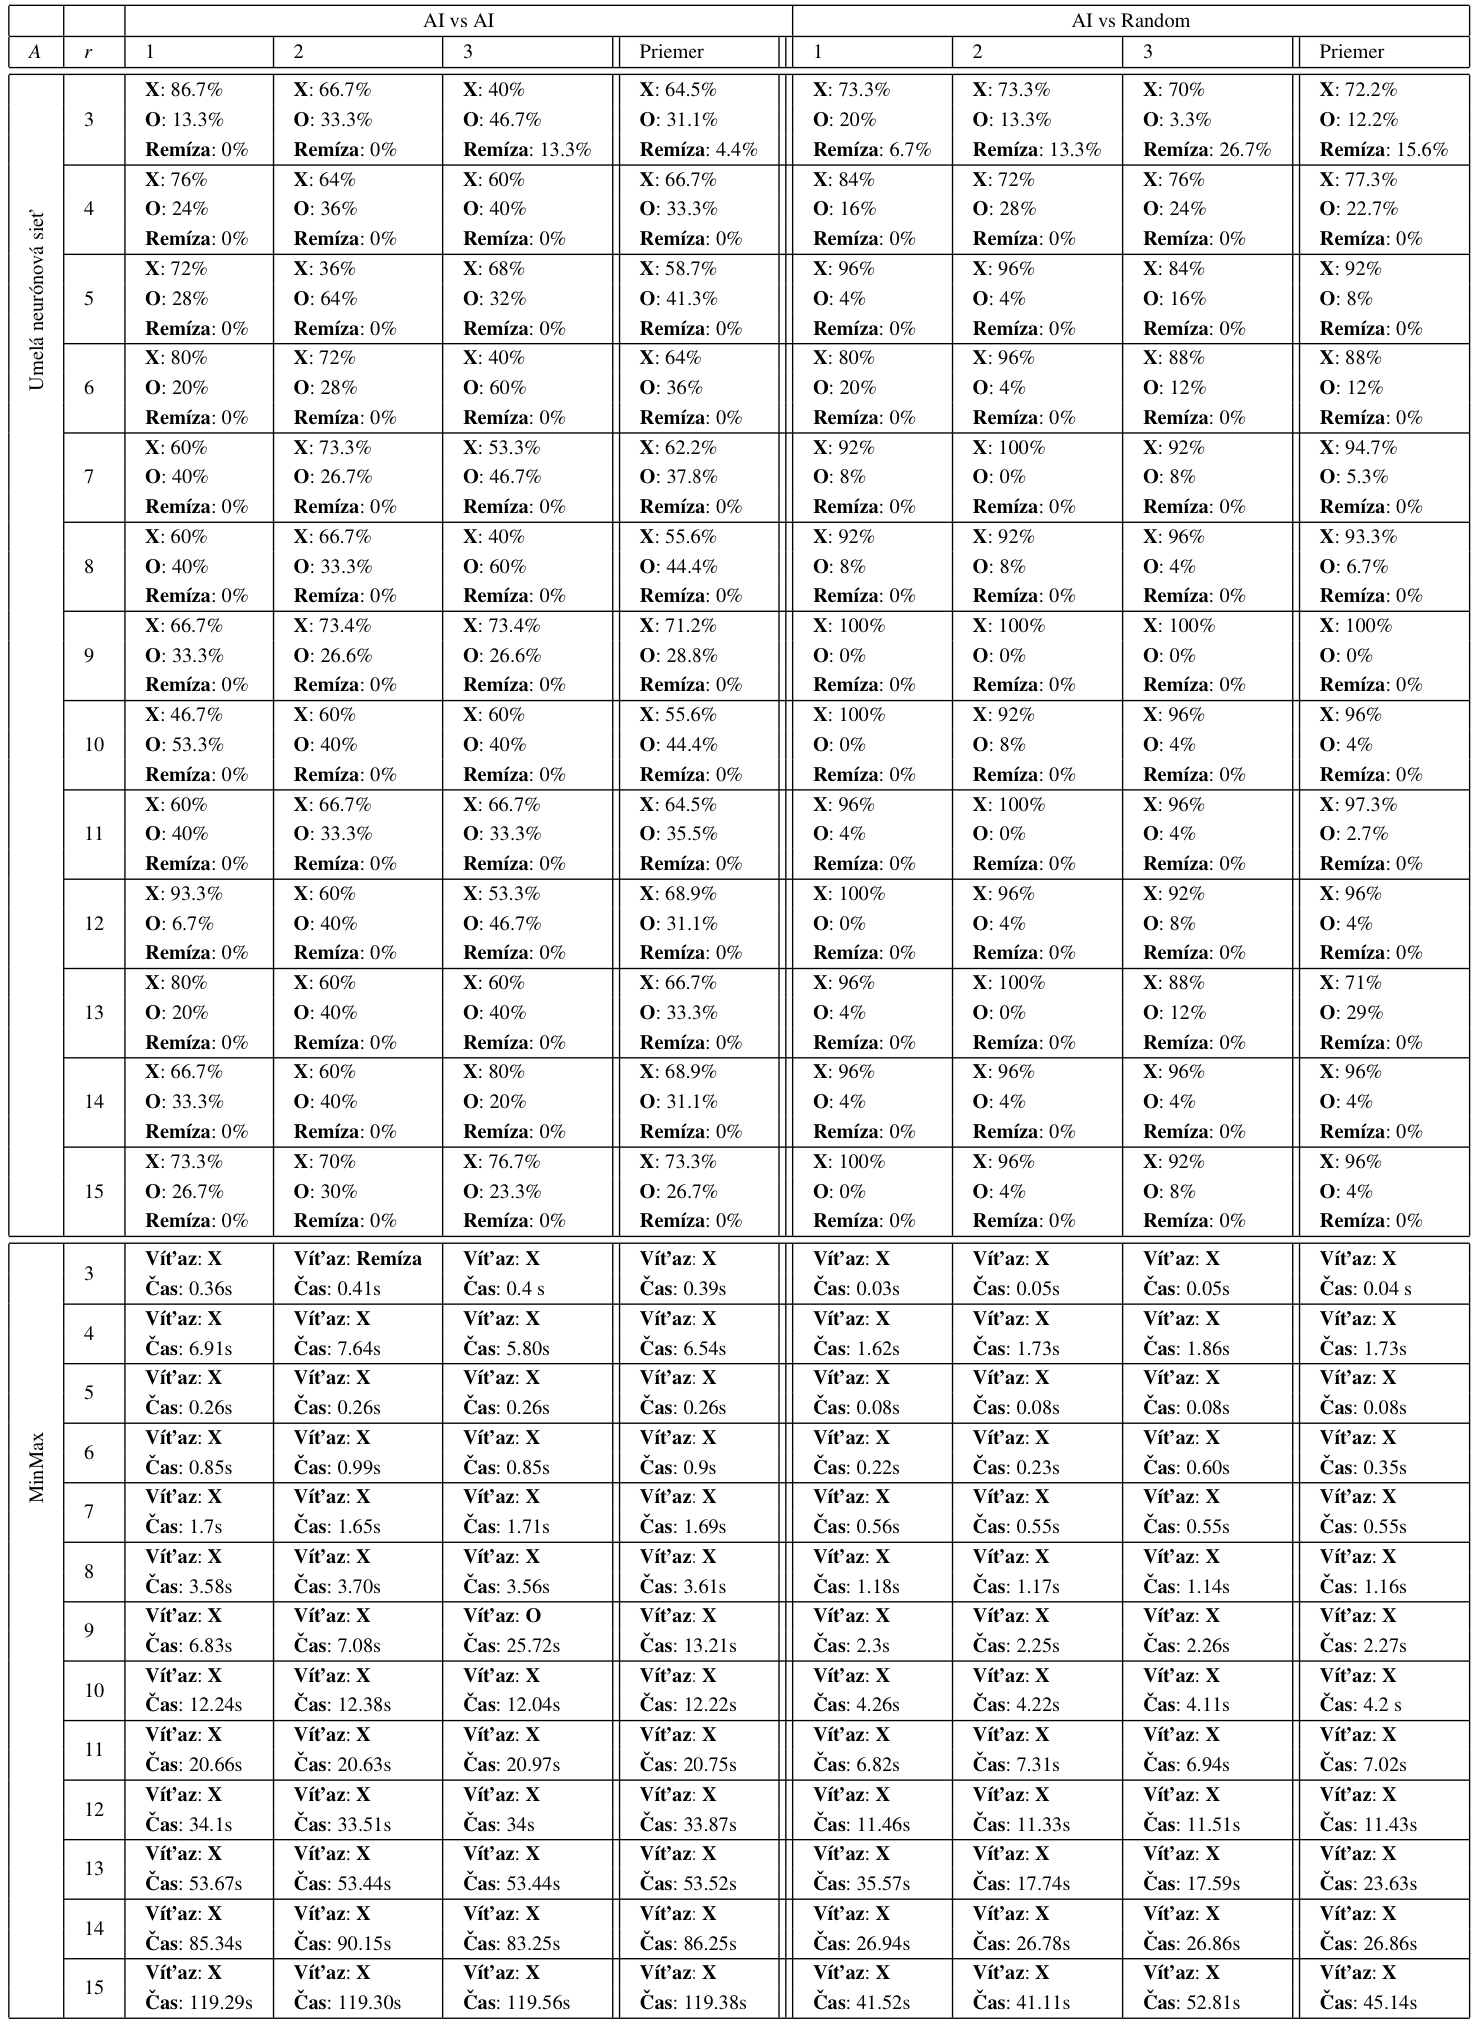
\includegraphics[width=1\textwidth]{images/table.png}
    \end{figure}
    \caption{Výsledky experimentov s rôznymi veľkosťami}\label{table:experiments-boards}
\end{table}
\clearpage

\paragraph{Vyhodnotenie výsledkov}

Pri algoritme minimax je zjavné, že je to exaktný algoritmus, pretože časy jednotlivých hier hlavne pri vyšších
rozmeroch boli extrémne veľké (pričom maximálna hĺbka stromu pri $i>2$ bola nastavená na $l=2$) a rástli exponenciálne.
Aj keď vo variante s náhodným ťahom oponenta sú časy značne nižšie, sú stále veľmi vysoké pre reálne použitie.

Výsledky metódy umelých neurónových sietí boli v prípade variantu, kde proti sebe hrala tá istá neurónová sieť
približne rovnaké so vstupnými údajmi a teda so simuláciami náhodných hier.
Z týchto výsledkov je možné usúdiť, že sieť je natrénovaná veľmi dobre a dokonca pri variante s náhodnými ťahmi oponenta
bola v drvivej väčšine prípadov úspešná.
Znamená to, že táto umelá neurónová sieť by mala byť úspešná vo väčšine prípadov pri hre so sofistikovanejším oponentom.

\subsection{Experimenty s rôznymi modelmi}\label{subsec:experiments-versus}
Tieto typy experimentov boli vykonávané na ploche s veľkosťou $10 \times 10$ s počtom znakov potrebných pre výhru 3
(resp. $r = 10$, $w = 3$ a $d = 2$), pričom použité boli 3 algoritmy:
\begin{itemize}
    \item Umelá neurónová sieť popísaná v \autoref{subsec:algo-ann}.
    Táto sieť slúžila ako hlavný algoritmus pre cieľového hráča a bola porovnávaná s nasledujúcimi dvoma algoritmami
    \item Algoritmus minimax
    \item Nasledujúca neurónová sieť:\cite{first_ann}
    \begin{itemize}
        \item na vstupe je 200 neurónov a za vstup pokladá vektor $v$ (v prípade experimentu je $|v|=100$)
        \item \enquote{dropout} vrstva, ktorá s pravdepodobnosťou 0.2 nepoužije vstup do nasledujúcej vrstvy (\enquote{zahodí ho})
        \item vrstva s počtom neurónov 125
        \item vrstva s počtom neurónov 75
        \item \enquote{dropout} vrstva, ktorá s pravdepodobnosťou 0.1 nepoužije vstup do nasledujúcej vrstvy
        \item vrstva s počtom neurónov 25
        \item na výstupe je \enquote{one-hot} array vyjadrujúce, ktorý z hráčov vyhral (\textbf{X}, \textbf{O}) alebo či nastala remíza
    \end{itemize}
\end{itemize}

\clearpage
\begin{table}[H]
    \centering
    \begin{tabular}{|l|l|l|l||l|}
        \hline
        \multirow{2}{*}{} &
        \multicolumn{3}{c|}{Experiment č.} & \\
        \hline
        \textit{M} & 1 & 2 & 3 & Priemer \\
        \hline
        \hline
        \multirow{3}{*}{\small\rotatebox[origin=c]{90}{MinMax}}
        & \textbf{X}: 0\% & \textbf{X}: 0\% & \textbf{X}: 0\% & \textbf{X}: 0\% \\
        & \textbf{O}: 100\% & \textbf{O}: 100\% & \textbf{O}: 100\% & \textbf{O}: 100\% \\
        & \textbf{Remíza}: 0\% & \textbf{Remíza}: 0\% & \textbf{Remíza}: 0\% & \textbf{Remíza}: 0\% \\
        \hline
        \multirow{3}{*}{\small\rotatebox[origin=c]{90}{ANN}}
        & \textbf{X}: 95\% & \textbf{X}: 100\% & \textbf{X}: 100\% & \textbf{X}: 98.3\% \\
        & \textbf{O}: 5\% & \textbf{O}: 0\% & \textbf{O}: 0\% & \textbf{O}: 1.7\% \\
        & \textbf{Remíza}: 0\% & \textbf{Remíza}: 0\% & \textbf{Remíza}: 13.3\% & \textbf{Remíza}: 0\% \\
        \hline
    \end{tabular}
    \caption{Výsledky experimentov s rôznymi modelmi}\label{table:experiments-versus}
\end{table}

\paragraph{Experimenty s rôznymi modelmi}

Napriek tomu, že umelá neurónová sieť bola úspešná pri hre s inou umelou neurónovou sieťou, nevyrovná sa to exaktnému
algoritmu minimax, pri ktorom úplne pohorela.
Ak ale je cieľom efektivita, nie je možné použiť algoritmus minimax vzhľadom na čas, ktorý algoritmus potrebuje pre
vykonanie výpočtov.

\subsection{Celkové vyhodnotenie}\label{subsec:results-analysis}

Umelá neurónová sieť navrhnutá v \autoref{subsec:algo-ann} bola oproti externej umelej neurónovej sieti úspešnejšia, no
na druhej strane je citeľne slabšia v hre s exaktným algoritmom (minimax).
Implementovaná štruktúra má silnú šancu vyhrať nad oponentom s náhodným výberom a menšiu (no stále pravdepodobnejšiu)
šancu vyhrať v hre s inteligentným oponentom na rôznych plochách.
Pravdepodobnosť výhry sa v tomto prípade dá zvýšiť zväčšením vzorky dát, s ktorými umelá neurónová sieť pracuje
(trénuje).
